\subsection{随机工作负载下的性能评估}
\label{subsec:sgxdedup-synthetic}

本文使用一组随机文件组成一个随机工作负载数据集,其中每个文件均仅包含全数据集范围内非重复的数据块(完全随机)。 默认情况下,本文将随机文件大小设置为2\,GB(Exp\#2除外,本文在其中对消息锁加密密钥生成性能进行了压力测试)。 客户端通过云服务端上传或下载文件。为了避免磁盘I/O对性能的影响,本文将随机文件存储在内存中而不是磁盘上(Exp\#7除外,本文在真实云环境部署中使用磁盘处理随机文件数据集)。本文的结果为10次运行的平均结果以及T分布(\textit{ Student's t-Distribution})下的95\%置信区间包含在条形图中(为简洁起见,本文在折线图中不标注置信区间)。

\paragraph*{Exp\#1(单客户端消息锁加密密钥生成)。}本文评估\sysnameS 中两轮消息锁加密密钥生成的效率。首先,客户端基于Rabin指纹(\S\ref{sec:sgxdedup-implementation})对2\,GB随机文件进行可变长度分块,并产生数据块指纹,发出消息锁加密密钥生成请求。然后,客户端为另一个2\,GB随机执行相同步骤进行密钥生成。不同之处在于第二轮密钥生成将使用预先计算的加解密掩码加速密钥安全区处理(\S\ref{subsec:sgxdedup-encryption})。

本文将\sysnameS 的单客户端消息锁加密密钥生成速度与现有服务器辅助密钥生成方案进行了对比。本文考虑两种基于OPRF协议的密钥生成方法,即 \textit{OPRF-BLS}\cite{armknecht2015transparent}和\textit{ OPRF-RSA}\cite{bellare2013DupLESS},它们分别基于盲BLS签名和盲RSA签名实现了OPRF原语(\S\ref{subsec:sgxdedup-problem})。此外,本文还考虑了两种较宽松的密钥生成方法,即\textit{MinHash encryption}\cite{qin17}和\textit{TED}\cite{li2020TED},它们以存储效率和安全性为代价换取密钥生成性能。具体来说,MinHash encryption使用OPRF-RSA协议基于每个数据段(较数据块更大的单位,平均大小为1\,MB)中所有数据块指纹的最小值产生消息锁加密密钥。TED使用数据块的短哈希、密钥服务器的全局秘密以及基于草图(Sketch)统计的数据块频率共同为每个数据块生成消息锁加密密钥(参见\cite{li2020TED}中的\S3.3)。

\begin{figure}[!htb]
    \centering
    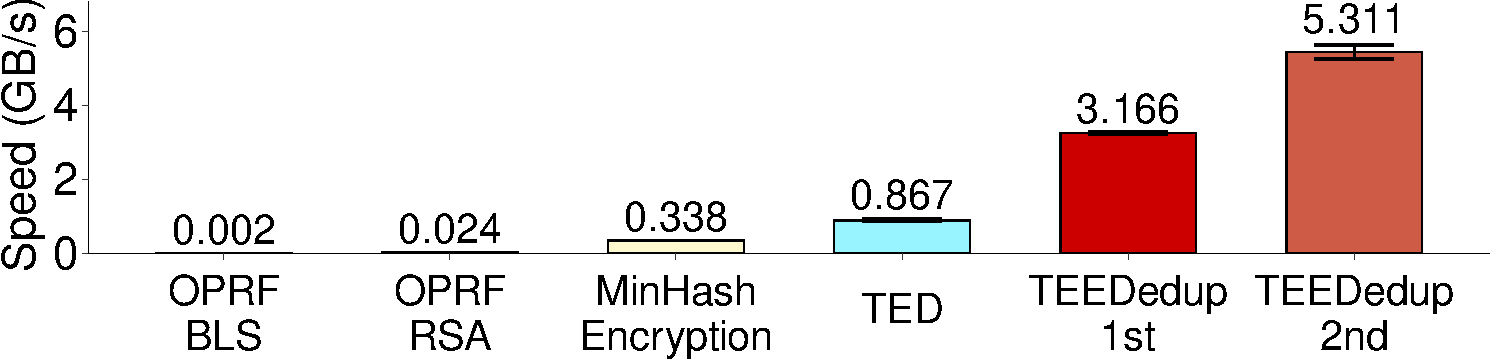
\includegraphics[width=0.8\textwidth]{pic/sgxdedup/expa2_keyGenPerformance.pdf}
    \caption{(Exp\#1)单客户端消息锁加密性能对比}
    \label{fig:sgxdedup-keygen-comparison}
\end{figure}

图~\ref{fig:sgxdedup-keygen-comparison}显示了测试结果。\sysnameS 通过避免OPRF-BLS、OPRF-RSA和MinHash encryption中昂贵的密码原语以及TED中的频率计数等计算,实现了远超所有对比对象的密钥生成性能。\sysnameS 的第一轮密钥生成相比OPRF-BLS和OPRF-RSA实现了1,583倍和131.9倍的性能提升。与MinHash encryption和TED(两者均牺牲了部分存储效率和安全性)相比,分别提高了9.4倍和3.7倍。而第二轮基于推测性加密,\sysnameS 将第一轮的消息锁加密密钥生成速度再次提高了67.8\%。

\paragraph*{Exp\#2(多客户端消息锁加密密钥生成)。}为了对密钥生成安全区的密钥生成性能进行压力测试,本文采用一台设备通过多线程模拟福哦个客户端,同时向密钥服务器(在不同的设备上运行)发出消息锁加密密钥生成请求。这里,每个模拟客户端仅包含一个线程用于发出密钥生成请求(随机生成数据块指纹)。

由于密钥安全区中可存储的加解密掩码至多可用于处理约11.25\,GB的原始数据(\S\ref{subsec:sgxdedup-encryption}),为了在第二轮密钥生成中为每个模拟的客户端均启用推测行加密,本文将将每个模拟客户端配置为生成40,960个指纹(约满足320\,MB原始数据的密钥生成需求),并将密钥安全区离线计算加解密掩码的客户端数量配置为与模拟客户端数量一致。使得第二轮密钥生成中,所有客户端的所有密钥生成请求均通过推测行加密进行处理。本文统计分析所有模拟客户端聚合的密钥生成速度,该速度定义为总密钥生成数量除以第一个客户端启动到所有客户端全部完成密钥生成的时间。

\begin{figure}[!htb]
    \small
    \centering
    \begin{tabular}{@{}c@{}c@{}c}
        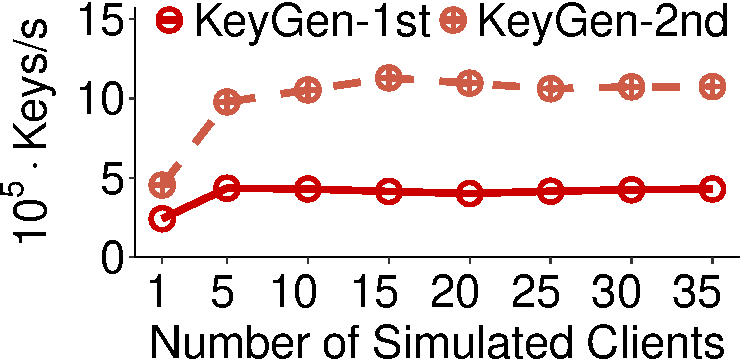
\includegraphics[width=0.49\textwidth]{pic/sgxdedup/expa3_keyScale_performance_number_singleThread.pdf} &
        \hspace{5pt}
        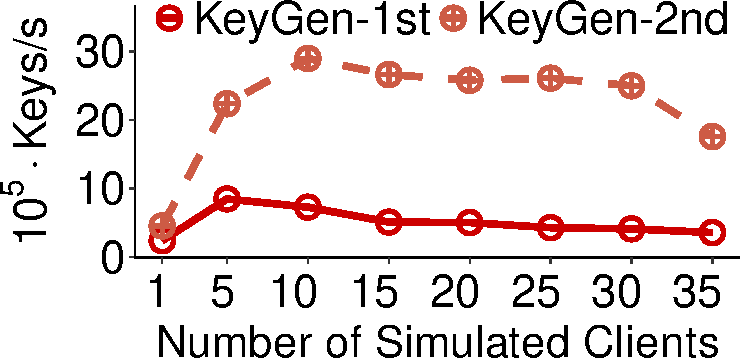
\includegraphics[width=0.49\textwidth]{pic/sgxdedup/expa3_keyScale_performance_number_multiThread.pdf}\\
        \mbox{\small (a)密钥安全区单线程执行} &
        \mbox{\small (b)密钥安全区多线程执行}\\
    \end{tabular}
    \caption{(Exp\#2) 多客户端消息锁加密密钥生成} 
    \label{fig:sgxdedup-exp-keygen-scalability}
\end{figure}

图~\ref{fig:sgxdedup-exp-keygen-scalability}(a)显示了密钥安全区仅使用单个线程处理所有模拟客户端的密钥生成请求时的聚合密钥生成速度。在第一轮和第二轮密钥生成中,\sysnameS 分别在5个和15个客户端时达到最大生成速度($4.3\times 10^5$\,keys/s和$11.3\times 10^5$\,keys/s)。随后,受限于单核处理能力上限,密钥生成速度基本保持不变。图~\ref{fig:sgxdedup-exp-keygen-scalability}(b)显示了密钥安全区多线程服务模拟客户端时的密钥生成聚合速度。第一轮和第二轮密钥生成分别在5个和10个模拟客户端时实现了最高$8.5\times 10^5$\,keys/s和$29\times 10^5$\,keys/s的密钥生成速度,随后由于CPU上下文切换开销逐渐增大,聚合速度逐渐下降。平均而言,第二轮基于推测行加密相较于第一轮实现了4.4倍的的聚合密钥生成加速。

\paragraph*{Exp\#3(密钥生成批量大小的影响)。}

本文首先使用Exp\#1的方法来评估请求密钥生成的指纹批量大小对密钥生成速度的影响。图~\ref{fig:sgxdedup-exp-keygen-breakdown}(a) 显示了两轮密钥生成速度与请求的指纹批量大小的关系。当指纹批量大小从$1$更改为$2^{15}$时,第一轮和第二轮的密钥生成速度分别从0.0086\,GB/s增加到3.3\,GB/s以及从0.0091\,GB/s增加到6.5\,GB/s。图~\ref{fig:sgxdedup-exp-keygen-breakdown}(b)去除网络传输开销后分别统计了客户端及密钥安全区在生成1\,MB原始数据的消息锁加密密钥时分别的计算开销。密钥安全区和客户端的时间消耗随着指纹批量的增大而减少,这是因为更大的批量大小意味着要为所有指纹批次计算的MAC更少(参见\S\ref{sec:sgxdedup-implementation})。此外,密钥安全区的时间开销随着批量大小增加在第一轮中从2.0\,ms减少到0.2\,ms,在第二轮从 1.8\,ms减少到0.1\,ms。时间开销明显减少的原因是较大的指纹批量大小避免了过多次调用密钥生成安全区内调用(key generation Ecall),并减少了CPU的上下文切换开销。

\begin{figure}[!htb]
\centering
\begin{tabular}{@{\ }c@{\ }c}
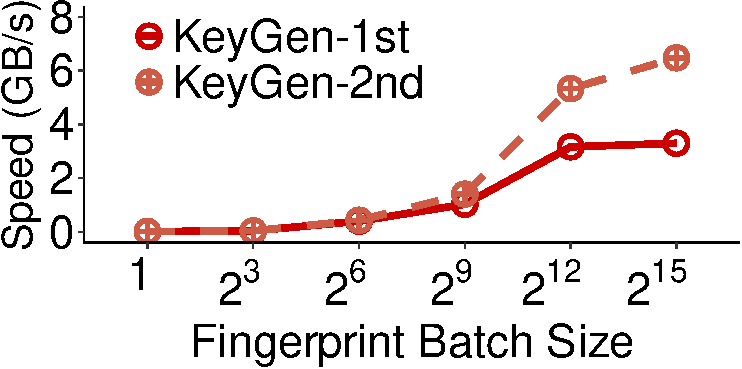
\includegraphics[width=0.48\textwidth]{pic/sgxdedup/expa2_keyEnclaveBatchSize_Performance_overall.pdf}                                         &
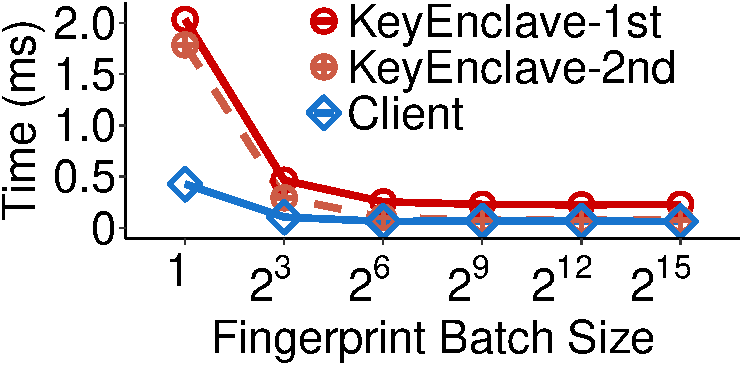
\includegraphics[width=0.48\textwidth]{pic/sgxdedup/expa2_keyEnclaveBatchSize_Performance_1st.pdf}                                               \\
\mbox{\parbox{0.48\textwidth}{\small (a) 总体密钥生成速度vs.批量大小}} &
\mbox{\parbox{0.48\textwidth}{\small (b) 密钥生成中的计算开销vs.批量大小}}
\end{tabular}
\caption{(Exp\#3)指纹批量大小对密钥生成性能的影响}
\label{fig:sgxdedup-exp-keygen-breakdown}
\end{figure}


\paragraph*{Exp\#4(自会话密钥的更新延迟)。} 

在自更新会话密钥管理中,密钥安全区和云服务端通过密钥回归独立地执行密钥更新,其方法是从旧密钥状态导出新密钥状态(\S\ref{subsec:sgxdedup-key-management})。本文评估密钥安全区和云服务端中的密钥更新延迟。

\begin{figure}[!htb]
    \centering
    \begin{tabular}{@{\ }c@{\ }c}
    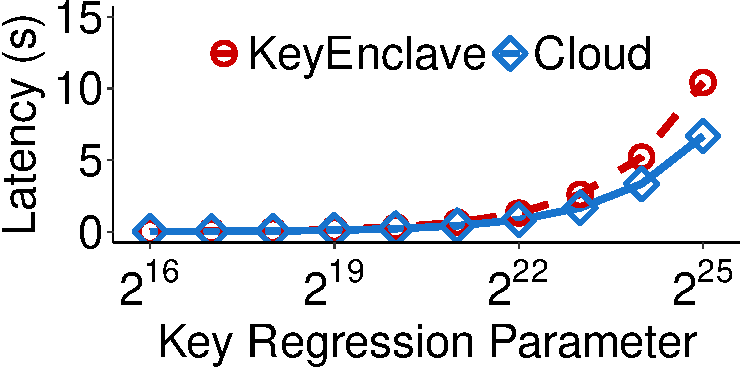
\includegraphics[width=0.48\textwidth]{pic/sgxdedup/expa5_keyRegression_time.pdf} &
    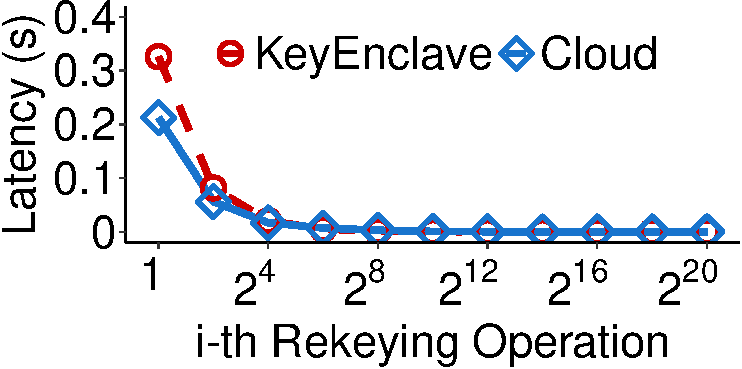
\includegraphics[width=0.48\textwidth]{pic/sgxdedup/expa5_keyRegression_time_default.pdf} \\
    \mbox{\small (a) For different parameters} &
    \mbox{\small (b) For different occurrences}
    \end{tabular}
    \caption{(Exp\#4)会话密钥更新延迟}
    \label{fig:sgxdedup-rekeyingLatency}
\end{figure}
    
图~\ref{fig:sgxdedup-rekeyingLatency}(a)显示了会话密钥的首次更新延迟与密钥回归参数(即,可承受的最大密钥更新次数,参见\S\ref{subsec:sgxdedup-key-management})的关系。密钥安全区和云服务端的密钥首次密钥更新延迟随着密钥回归参数的增大而增加,因为更大的密钥回归参数意味着密钥更新中的哈希计算更多。由于安全区处理密集计算的能力较弱\cite{harnik2018SGX},这里密钥安全区的密钥更新延迟相较云服务端高1.22-1.56倍。

图~\ref{fig:sgxdedup-rekeyingLatency}(b)显示了每次会话密钥更新操作的延迟,此时初始化的密钥回归参数固定为2$^{20}$。随着执行更多的密钥更新操作,密钥更新延迟逐渐减少,每次密钥更新操作均可相较于上一次密钥更新操作节省一次哈希计算。平均而言,密钥安全区的密钥更新延迟为0.040\,s。相比之下,云服务端约为0.027\,s,这意味着密钥更新开销是有限的。

\paragraph*{Exp\#5 (数据所有权证明计算开销)。}本文评估\sysnameS 的数据所有权证明性能。本文考虑一个对2\,GB随机文件执行数据所有权证明的客户端。客户端从该文件中创建明文数据块,加密每个明文数据块,并向云服务端发出数据所有权证明请求。本文根据客户端(所有权证明安全区对密文数据块计算指纹并产生相应签名)和云服务端(验证指纹对应的数据的真实性)中所有数据块的总计算时间来测量所有权证明计算开销。本实验中的速度计算排除了客户端和云服务端之间的网络传输时间开销(本文在Exp\#10中考虑了网络传输时间)。

本文将\sysnameS 与两种最先进的数据所有权证明方法进行比较:(i)\textit{PoW-MT}\cite{halevi11}(halevi等人提出的基本版本),该数据所有权证明方法使用纠删码对块进行编码,并在编码的内容上构建默克尔树用于所有权证明;(ii)\textit{PoW-UH}\cite{xu2013weak}建立在通用哈希之上,相较于PoW-MT牺牲部分安全性以换取更高的性能。为了公平比较,本文使用C++复现了PoW-MT和PoW-UH方法。此外,halevi等人\cite{halevi11}提出了改进的数据所有权证明方法,但它们均为了更低的内存开销产生了更大的性能开销。

\begin{figure}[!htb]
    \begin{minipage}[t]{0.47\textwidth}
        \centering
        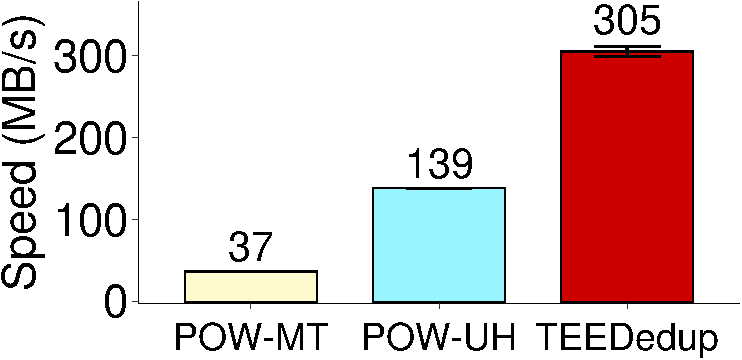
\includegraphics[width=\linewidth]{pic/sgxdedup/expa4_powPerformance.pdf}
        \caption{\small(Exp\#5)数据所有权证明的计算性能}
        \label{fig:sgxdedup-pow-comparison}
        \end{minipage}%
    \hspace{0.2in}
    \begin{minipage}[t]{0.47\textwidth}
        \centering
        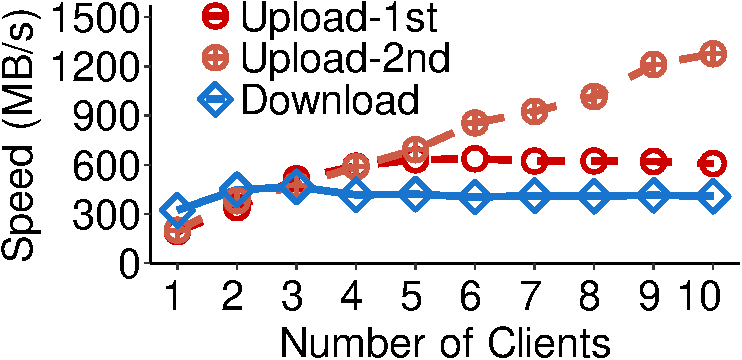
\includegraphics[width=\linewidth]{pic/sgxdedup/expb1_multiple_client.pdf}  
        \caption{(Exp\#8) Multi-client uploads and downloads.}
        \label{fig:sgxdedup-multiClientThroughput}
    \end{minipage}%
\end{figure}

图~\ref{fig:sgxdedup-pow-comparison}显示了性能测试结果。由于\sysnameS 避免了客户端中的纠删码编码和默克尔树构造,其实现了相较于PoW-MT高达8.2倍的性能提升。此外,\sysnameS 相较于安全性较弱的PoW-UH实现了2.2倍的性能提升。


%TODO
\paragraph*{Exp\#10 (密文数据块批量大小对性能的影响)。} 本文现在评估密文数据块批大小对 \sysnameS 的 PoW 性能的影响。与 Exp\#5 中考虑的计算 PoW 速度相反,本文测量 \textit{ 有效 PoW 速度},作为文件大小(即 2\,GB)与从 所有权证明安全区开始的总时间的比率计算密文数据块的指纹,直到云验证所有指纹。本文禁用客户端的上传操作和云服务端的重复数据删除操作,以减轻性能噪音。

图~\ref{fig:sgxdedup-exp-pow-impact}(a) 显示了有效 PoW 速度与不同批量大小的关系。本文看到有效 PoW 速度随着密文批量大小从 6.2\,MB/s 到 360.9\,MB/s 的增加而增加。图~\ref{fig:sgxdedup-exp-pow-impact}(b) 显示了所有权证明安全区和云在 PoW 中每次操作 1\,MB 数据时的相应计算时间。云的消耗时间很低(例如,低于 0.05\,ms),而 所有权证明安全区的时间随着批量大小从 4.1\,ms 减少到 2.7\,ms,因为减少了上下文切换开销(见 Exp \#10)。请注意,即使批量密文数据块的总大小超过 EPC 大小,所有权证明安全区仍保持高计算性能,因为它不需要将数据内容复制到安全区(\S\ref{sec:sgxdedup-implementation})。

\begin{figure}[!htb]
\centering
\begin{tabular}{@{\ }c@{\ }c}
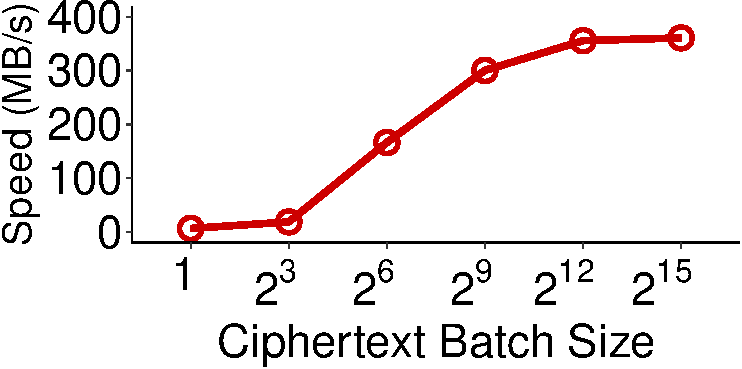
\includegraphics[width=0.48\textwidth]{pic/sgxdedup/expa4_powBatchSize_overall.pdf} &
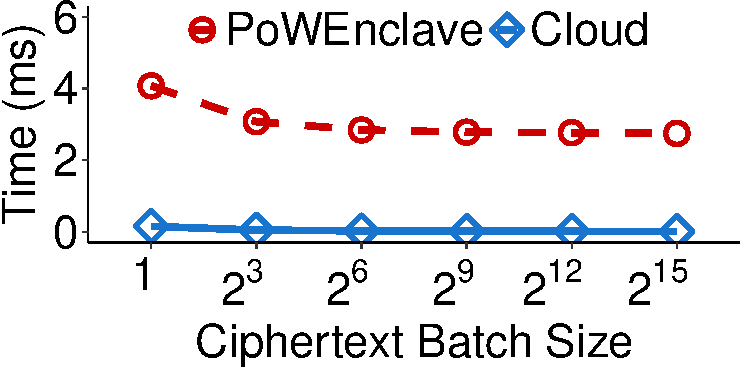
\includegraphics[width=0.48\textwidth]{pic/sgxdedup/expa4_powBatchSize_breakdown.pdf}                 \\
\mbox{\parbox{0.48\textwidth}{\small (a) Effective PoW speed vs. ciphertext batch size
}}                                                                 &
\mbox{\parbox{0.48\textwidth}{\small (b) Computational time per processing 1\,MB data}}
\end{tabular}
\caption{(Exp\#10) Impact of ciphertext batch size to PoW performance.}
\label{fig:sgxdedup-exp-pow-impact}
\end{figure}


\paragraph*{Exp\#6 (单客户端上传及下载性能)} 本文考虑单个客户端,并将 \sysnameS 的上传和下载性能与两个基线系统进行比较:(i) \textit{ PlainDedup},禁用 \sysnameS 的密钥生成、加密和PoW操作,从而实现源端重复数据删除,无需任何安全保护; (ii) \textit{ {\em DupLESS}} \cite{bellare2013DupLESS},它通过 OPRF-RSA 生成每块 消息锁加密 密钥,执行加密并将所有密文数据块上传到云以进行重复数据删除。由于 {\em DupLESS} 的原始实现不提供重复数据删除存储后端(假设使用了 Dropbox),本文根据 \cite{bellare2013DupLESS} 中描述的设计在 C++ 中实现 {\em DupLESS}。请注意,PlainDedup 基于未加密的文件元数据检索文件,并且不同于加密后重复数据删除系统中的两轮下载(即 \sysnameS 和 {\em DupLESS});在后者中,客户端首先下载并解密文件元数据,然后下载块以重建文件 (\S\ref{subsec:sgxdedup-problem})。

本文分三个步骤评估上传和下载速度: (i) 客户端首先上传 2\,GB 文件; (ii) 客户端重新启动,然后上传另一个与前一个相同的 2\,GB 文件; (iii) 客户端下载文件。请注意,第二次上传执行源端重复数据删除(对于 PlainDedup 和 \sysnameS),并利用预先计算的掩码来加速密钥生成(仅适用于 \sysnameS)。


\begin{figure}[!htb]
    \centering
    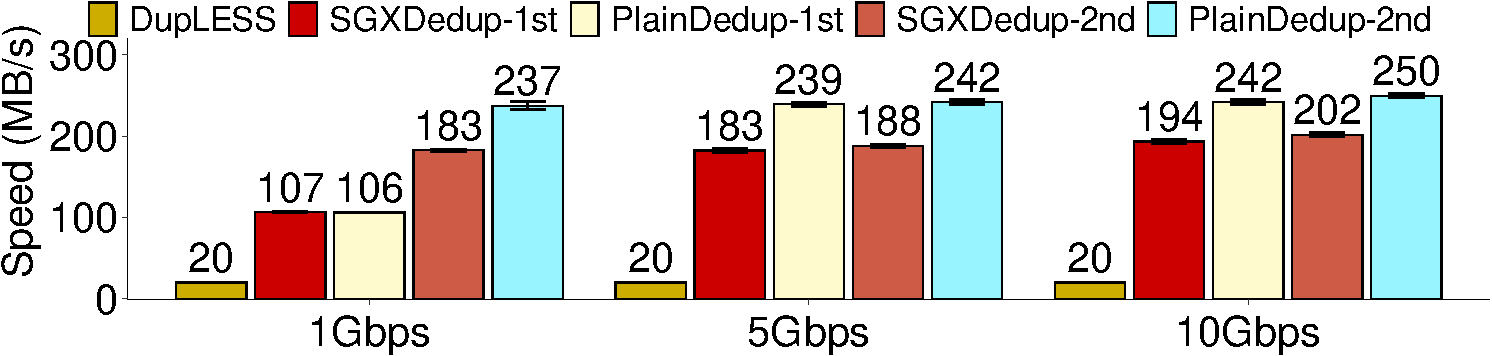
\includegraphics[width=0.64\textwidth]{pic/sgxdedup/upload_network_speed_bar.pdf} \ \ 
    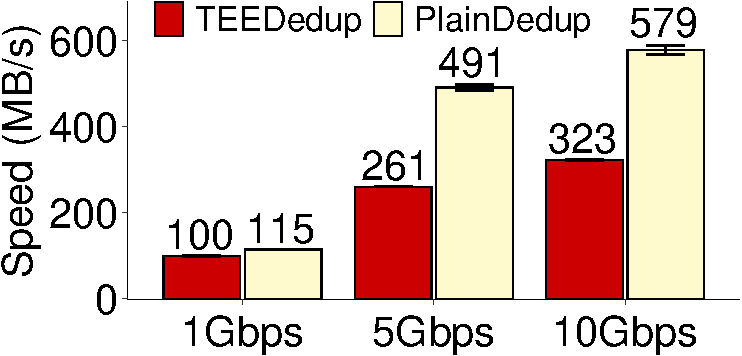
\includegraphics[width=0.32\textwidth]{pic/sgxdedup/download_network_speed_bar.pdf}
    \vspace{-3pt}\\
      \hspace{1.1in} {\small (a) Upload} \hspace{1.9in}
    {\small (b) Download}
    \vspace{-6pt}\\
    \caption{(Exp\#5) Single-client uploads and downloads. We exclude the second upload speed of {\em DupLESS} (which has the same performance in two uploads) and the download speed of {\em DupLESS} (which is identical to that of  \sysnameS).}
    \label{fig:sgxdedup-singleClientThroughput}
\end{figure}

图~\ref{fig:sgxdedup-singleClientThroughput}(a) 显示了由 {\tt trickle} \cite{eriksen05} 控制的不同网络带宽的上传速度。第一次上传,当网络带宽为 1\,Gbps 时,\sysnameS (106.6\,MB/s) 和 PlainDedup (106.2\,MB/s) 的上传速度均受网速约束,而性能{\em DupLESS} (20.1\,MB/s) 的瓶颈是基于 OPRF-RSA 的密钥生成 (Exp\#1)。当网络带宽增加到 10\,Gbps(默认)时,\sysnameS 和 PlainDedup 的上传速度分别达到 193.6\,MB/s 和 242.0\,MB/s,而 {\em DupLESS} 的上传速度稳定在 20.0\, MB/秒。对于第二次上传,由于其密钥生成性能瓶颈,{\em DupLESS} 达到了与第一次上传相同的速度。 \sysnameS 和 PlainDedup 的上传速度受网络带宽的影响较小,因为它们不需要传输数据。平均而言,\sysnameS 在第一次和第二次上传中分别比 {\em DupLESS} 实现了 8.1$\times$ 和 9.6$\times$ 的加速。即使与不安全的 PlainDedup 相比,\sysnameS 也只会导致相应的上传速度下降约 17.5\% 和 21.4\%。开销来自 \sysnameS 的安全机制,包括密钥生成、加密和 PoW。

图~\ref{fig:sgxdedup-singleClientThroughput}(b) 显示了下载速度。随着网络带宽增加到 10\,Gbps,\sysnameS 和 {\em DupLESS} 均达到 323.1\,MB/s,比 PlainDedup 下降了 44.2\%。原因是他们连续检索和解密文件元数据,然后下载密文数据块。

\paragraph*{Exp\#7(真实云上传和下载)。} 本文现在扩展 Exp\#5 并评估真实云部署中的上传和下载速度。具体来说,本文将客户端和密钥服务器部署在本文的局域网测试平台(\S\ref{sec:sgxdedup-evaluation})中,并通过互联网将客户端连接到\textit{ 阿里云},本文在其中租用了一个虚拟机\textit{ ecs.c6e.xlarge} 运行云。云机配备四核3.2GHz CPU(其主机平台为Intel Xeon Cascade Lake Platinum 8269CY),8GB内存。本文以 \textit{ Alibaba General Purpose NAS} 作为存储后端来挂载云。 NAS 可以实现高达 20000\,IOPS 的 4\,K 次随机读写。

本文使用磁盘上的数据文件进行上传(与 Exp\#5 相对,后者在上传之前将文件加载到客户端的内存中),并允许云服务端将接收到的数据文件存储在 NAS 中。本文还使用 {\tt scp} 将整个数据文件(即 2\,GB)从客户端上传到云服务端,以提供互联网环境下的数据传输基准。


Table~\ref{tab:sgxdedup-real-cloud} 显示了结果。在第一次上传时,所有系统的性能(\sysnameS 为 11.4\,MB/s,PlainDedup 为 11.6\,MB/s,{\em DupLESS} 为 10.8\,MB/s)受限于 Internet 带宽(11.9\,MB/ s)。在第二次上传中,\sysnameS 实现了 104.3\,MB/s,与 {\em DupLESS} 相比加速了 9.7$\times$,与 PlainDedup 相比下降了 13.2\%。请注意,性能差异比 Exp\#5 中的要小,因为 \sysnameS 和 PlainDedup 现在受客户端磁盘 I/O 的限制。在下载中,这三个系统的性能再次受到 Internet 带宽的限制,而 \sysnameS 和 {\em DupLESS} 由于它们的串行检索和解密(Exp\#5),将 PlainDedup 的下载速度降低了 10.6\%。

\begin{table}[!htb]
\small
\centering
\renewcommand{\arraystretch}{1.05}
\begin{tabular}{cccc}
\toprule
{\bf 方案} & {\bf 第一轮上传(非重复数据)} & {\bf 第二轮上传(重复数据)} & {\bf 下载} \\
\midrule
网络带宽 & \multicolumn{3}{c}{11.9 $\pm$ 0.03} \\  
\sysnameS & 11.4 $\pm$ 0.3 & 104.3 $\pm$ 1.2 & 10.1 $\pm$ 0.1 \\ 
PlainDedup & 11.6 $\pm$ 0.1 & 120.1 $\pm$ 1.4 & 11.3 $\pm$ 0.3 \\
{\em DupLESS} & \multicolumn{2}{c}{10.8 $\pm$ 0.2}  & 10.1 $\pm$ 0.1 \\
\bottomrule
\end{tabular}
\caption{(Exp\#7) Real-cloud upload and download (unit: MB/s).} 
\label{tab:sgxdedup-real-cloud}
\vspace{-6pt}
\end{table}

\paragraph*{Exp\#8(多客户端上传和下载)。}本文现在考虑同时发布上传/下载的多个客户端。本文专注于 \sysnameS,并将密钥安全区配置为在第一次上传后为每个客户端同等地预先计算掩码。本文将网络带宽固定为 10\,Gbps,并评估所有客户端完成上传/下载的 \textit{ aggregate} 上传和下载速度。

图~\ref{fig:sgxdedup-multiClientThroughput} 显示了多达 10 个客户端的结果。第二轮的总上传速度随着客户端数量的增加而增加,达到1277.1\,MB/s。另一方面,由于客户端之间的写竞争,第一轮的总上传速度增加了七个客户端的 637.0MB/s,随后下降到 10 个客户端的 620.3MB/s。同样,由于多个客户端的读取竞争,总下载速度最终下降到 408.8\,MB/s。

\paragraph*{Exp\#9(时间分解)。} 本文提供 \sysnameS 的时间分解来研究不同步骤的性能。假设key enclave已经启动,本文关注单个客户端的初始化和上传过程。初始化过程启动客户端的所有权证明安全区。上传过程包括以下步骤: (i) \textit{ chunking},将输入文件划分为明文数据块; (ii) \textit{ fingerprinting-p},计算明文数据块的指纹; (iii) \textit{ key generation},从密钥安全区生成 消息锁加密 密钥; (iv) \textit{ encryption},加密明文数据块; (v) \textit{ fingerprinting-c},所有权证明安全区计算密文数据块的指纹; (vi) \textit{ 签名},所有权证明安全区计算指纹的签名; (vii) \textit{ 验证},其中云验证接收到的指纹的真实性; (viii) \textit{ deduplication},云检测重复的密文数据块并通知客户端; (ix) \textit{ transfer},上传非重复密文数据块和文件元数据。


\begin{table}[!htb]
\small
\centering
\setlength{\tabcolsep}{5pt}
\renewcommand{\arraystretch}{1.05}
\begin{tabular}{|c|c|c|c|}
\hline
  \multicolumn{2}{|@{\,}c|}{\textbf{Procedure/Step}} & \multicolumn{1}{l|}{\hspace{.5em}\textbf{First
  Upload}} &
\multicolumn{1}{c|}{\textbf{Second Upload}}                                                   \\ \hline \hline
\multicolumn{2}{|@{\,}c|}{Initialization}                   & 9.38 $\pm$
2.72\,s                                       & 0.80 $\pm$ 0.004\,s                       \\ \hline
\hline
                       \multicolumn{2}{|c|}{Chunking}                                 &
\multicolumn{2}{c|}{3.77 $\pm$ 0.15\,ms }                                                \\ \hline 
\multicolumn{2}{|c|}{Fingerprinting-p}
                                                           &
\multicolumn{2}{c|}{3.24 $\pm$ 0.28\,ms}                                                  \\ \hline
\multicolumn{2}{|c|}{Key generation}                     &
0.31 $\pm$ 0.01\,ms                           & 0.18
$\pm$ 0.01\,ms                                                                            \\ \hline
\multicolumn{2}{|c|}{Encryption} &
\multicolumn{2}{c|}{2.47 $\pm$ 0.10\,ms }                                                 \\ \hline
\multirow{3}{*}{PoW}  & Fingerprinting-c & \multicolumn{2}{c|}{3.28 $\pm$ 0.01\,ms }                                                 \\ \cline{2-4}
                      & Signing & \multicolumn{2}{c|}{0.01 $\pm$ 0.00004\,ms }                                                                                 \\ \cline{2-4}
                      & Verification & \multicolumn{2}{c|}{0.005 $\pm$ 0.00003\,ms } \\ \hline
                      \multicolumn{2}{|c|}{Deduplication}  & \multicolumn{1}{c|}{0.38 $\pm$ 0.03\,ms } & 0.48 $\pm$ 0.03\,ms  \\ \hline
                      \multicolumn{2}{|c|}{Transfer}  & \multicolumn{1}{c|}{1.29 $\pm$ 0.09\,ms } & 0.05 $\pm$ 0.01\,ms  \\ \hline
\end{tabular}
\caption{(Exp\#9) Time breakdown per 1\,MB of file data processed: fingerprinting-p and fingerprinting-c are operated on plaintext and ciphertext chunks, respectively.}
\label{tab:sgxdedup-system-breakdown}
\vspace{-6pt}
\end{table}

表~\ref{tab:sgxdedup-system-breakdown} 显示结果(每 1\,MB 处理的文件数据)。初始化过程在第一次上传时非常耗时,因为它需要联系Intel认证服务以检查所有权证明安全区的完整性。客户端再次重启时,不再需要执行远程认证,首轮设置时间减少91.5%。请注意,初始化过程的时间开销可以在多次上传和下载中分摊。


密钥生成步骤是高效的,最多占用整个上传时间的 2.1\%。通过推测性加密,\sysnameS 进一步将第一次上传的密钥生成时间减少了 41.9\%。此外,整个 PoW 步骤占用了总上传时间的 24.4\%,而 PoW 中的主要计算是密文数据块的指纹识别,这对于在加密后重复数据删除中查找重复项是必要的。通过轻量级的签名和验证步骤(最多占用总上传时间的 0.1\%),本文可以保护源端重复数据删除免受侧通道攻击,同时将首次上传的传输时间减少 96.1\%。

